\documentclass{article}[18pt]
\usepackage{../../../../format}
\lhead{A Level Maths - S3}

%File specific Preamble
\usepackage{enumitem} %Helps with lists in tables
\usepackage{pdfpages}
\usepackage{pdflscape}
\usepackage{setspace}
%File specific Preamble
\usepackage{multirow} %Merge cells in tables



\begin{document}
\begin{center}
\underline{\huge S3 Cheat Sheets}
\end{center}
\section{Combinations of random variables}
\subsection{Be able to combine two normally distributed variables}
$$E(X\pm Y)=E(X)\pm E(Y)$$
$$Var(X\pm Y)=Var(X)+Var(Y)$$
\textcolor{red}{Remember}
$$Var(2X)=2^2Var(X)$$
$$Var(X_1+X_2)=Var(X_1)+Var(X_2)=2Var(X)$$
None of this works for standard deviation, remember to square beforehand
\subsection{Be able to calculate $\mathbf{P(|X-Y|<k)}$ for some constant k}
$$P(|X-Y|<3)=P(-3<X-Y<3)=P(X-Y<3)-P(X-Y<-3)$$
\section{Sampling}
\subsection{Definitions}
Hypothesis - A statement concerning a population parameter\\ 
\\
Critical Region - The range of values that would lead to the rejection of $H_0$, and so the acceptance of $H_1$\\ 
\\
Statistic - A random variable, a function of known observations from a population, no unknown parameters\\ 
\\
Sampling unit - An individual unit of the population\\ 
\\
Sampling frame - A list of all sampling units\\ 
\\
Sampling distribution - All possible samples are chosen from the population\\ 
\\
Census - When every member of the population is investigated\\ 
\\
Hypothesis test - A mathematical procedure to examine a value of 
a population parameter proposed by the null hypothesis compared with an alternative hypothesis\\ 
\\
Population - A collection of all items\\ 
\\
Finite Population - One in which each individual member can be given a number\\ 
\\
Infinite population - One where it is impossible to number each individual member\\ 
\\
Significance level - The probability of incorrectly rejecting $H_0$\\ 
\\
Sample - A selection of items from a population\\ 

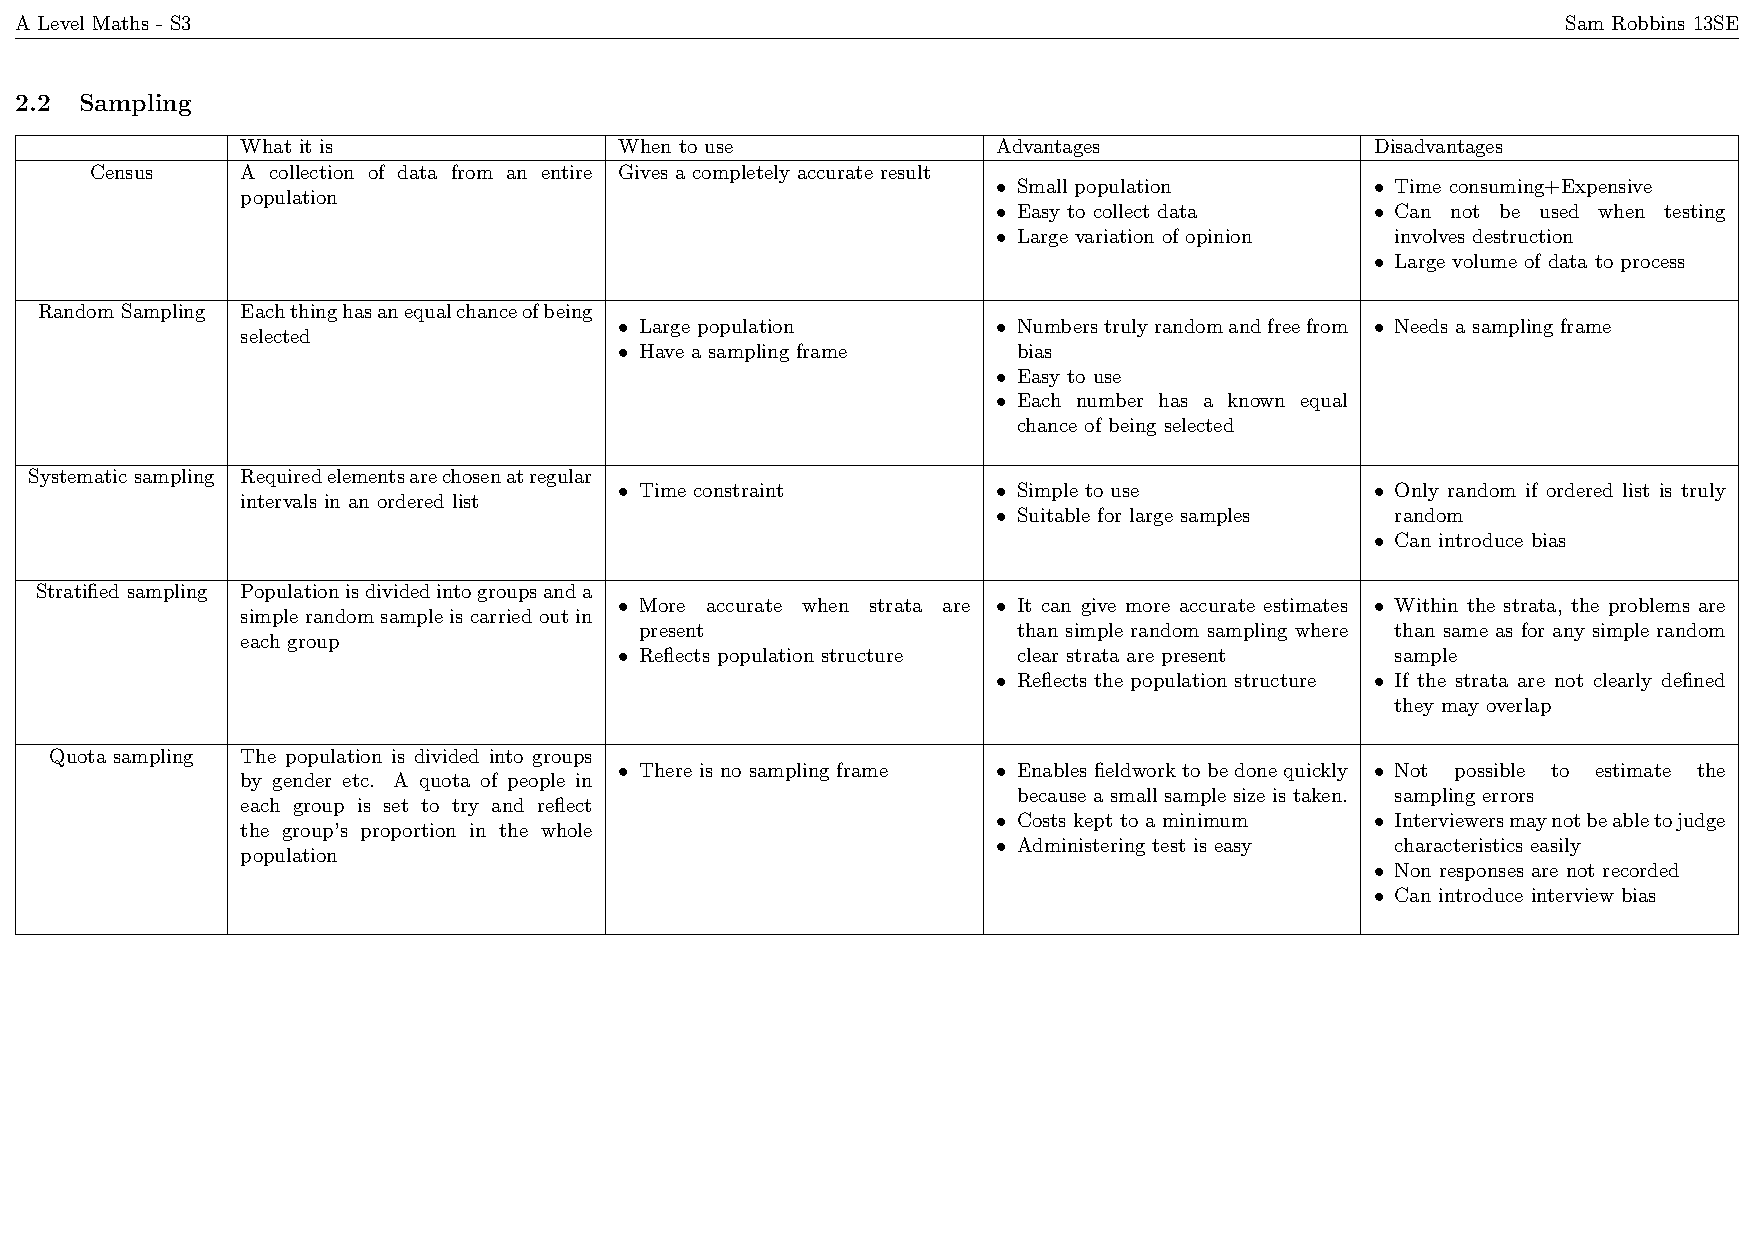
\includepdf[landscape=true]{Sampling2/Sampling2.pdf}
\newpage
\setcounter{subsection}{2}
\subsection{How to carry out samples}
\subsubsection{Simple random sampling}
\begin{itemize}
\item Allocate numbers to each member of the population
\item Use random number tables to select different numbers until enough have been selected
\item Members corresponding to the numbers become the sample
\end{itemize}
\subsubsection{Stratified sampling}
\begin{itemize}
\item Number the members in each strata
\item Use random numbers to select the members from each group
\item Number from each group in sample to be proportional to the number in the sample - calculate
\end{itemize}
\subsubsection{Systematic sampling}
\begin{itemize}
\item Randomly select first number between 1 and $Pop/sample$
\item Select every person at an interval of $Pop/sample$ after that
\end{itemize}
\subsubsection{Quota sampling}
\begin{itemize}
\item Non random sampling
\item Groups of the population
\end{itemize}
\section{Estimation, confidence intervals and tests}
\subsection{Know the definition of the central limit theorem}
\begin{itemize}
\item If $X_1,...,X_n$ is a random sample of size n, for large n
\item Drawn from the population of any distribution with mean $\mu$ and variance $\sigma^2$
\item The $\overline{X}$ is approximately $N(\mu,\frac{\sigma^2}{n})$
\end{itemize}
Most if this is under the sampling distributions header on the data sheet, just remember to include when n is large
\subsection{Know the definition of a statistic}
A random variable, a function of known observations from a population, no unknown parameters
\subsection{Understand what $\overline{X}$ is and find the distribution of $\overline{X}$}
$\overline{x}$ - Mean for a specific sample\\
$\overline{X}$  - A random variable allowing the sample mean to vary across different samples
$$\overline{X}\sim N\Bigg(\mu,\frac{\sigma^2}{n}\Bigg)$$
\textbf{Make sure when writing the distribution to use $\mu$, the population mean, rather than the sample mean}.
\subsection{Find value of n such that a value is in the confidence interval}
Use the formula:
$$\overline{X}\pm \times\frac{\sigma}{\sqrt{n}}$$
By setting this equal to a value, the value of n can be found such that the value will be in the confidence interval

\subsection{Find the minimum sample size required to have sufficient confidence that the sample mean lies in some range}
\textbf{Example}\\
$X\sim N(40,3^2)$. \textit{Find the minimum sample size such that the probability of the sample mean being greater than 42 is less than 5\%.}
$$\overline{X}\sim N\Bigg(40,\frac{9}{n}\Bigg)$$
$$P(\overline{X}>42)=P\Bigg(Z>\frac{42-40}{\frac{3}{\sqrt{n}}}\Bigg)$$
Find the C.V.
$$\frac{2}{\frac{3}{\sqrt{n}}}\geqslant1.6449\quad \Rightarrow n\geqslant6.087 \quad \therefore n=7$$
\subsection{Understand estimator notation}
$\hat{\mu}=\overline{x}$, anything with a hat on is an estimator
\subsection{Find the value of $S^2$}
$$S^2=\frac{\sum(X_i-\overline{X})^2}{n-1}$$
Replace the top of the fraction with $S_{xx}$
$$S^2=\frac{\sum x^2-\frac{(\sum x)^2}{n}}{n-1}$$
\subsection{Hypothesis test for the difference between means} 
When performing a hypothesis test for the difference between means, use the formula on the formula book:
$$\frac{(\overline{X}-\overline{Y})-(\mu_x-\mu_y)}{\sqrt{\frac{\sigma^2_x}{n_x}+\frac{\sigma^2_y}{n_y}}}$$
$H_0$ is always that the means are equal, or that they are equal with addition or subtraction to one\\
$H_1$ is always that one is greater, with the same addition or subtraction if stated in $H_0$
\subsection{State assumptions used to carry out a hypothesis test}
In general:
$$s^2=\sigma^2$$
Sample variance=Population variance
\subsection{Explain the relevance of the CLT}
It allows us to assume our means are normally distributed
\newpage
\section{Goodness of fit and Contingency tables}
\subsection{Goodness of fit method}
Method for testing goodness of fit:
\begin{enumerate}
\item Determine which distribution would conceptually be most appropriate
\item Set significance level
\item Estimate parameters (if necessary) from observed data
\item Form hypotheses $H_0$ and $H_1$
\item Calculate expected frequencies
\item Combine expected frequencies so that none are $<5$
\item Find degrees of freedom
\item Calculate critical value of $\chi^2$ from the table
\item Calculate $\sum\frac{(O_i-E_i)^2}{E_i}$
\item See if the value is significant and draw conclusion
\end{enumerate}
$X^2$ is distributed with a chi squared distribution $\chi^2_\nu$\\
Where $\nu=$ degrees of freedom\\
$$\textrm{The number of degrees of freedom}=\textrm{Number of classes (after combining)}-1$$
\\
$$\sum\frac{(O_i-E_i)^2}{E_i} \textrm{can be rewritten as  } \quad \Bigg(\sum\frac{O^2_i}{E_i}\Bigg)-N$$
$H_0$ is always that the distribution is a good model\\
$H_1$ is always that the distribution is not a good model
\subsubsection{Normal distribution}
When testing for a normal distribution the two ends of the table must extend to infinity to ensure that the probabilities add to 1
\subsubsection{Degrees of freedom}
The degrees of freedom starts as the number of columns, then 1 is subtracted from it for various reasons:
\begin{itemize}
\item Probabilities must add to 1 so one of the probabilities could be approximated
\item Approximation of p in binomial, or $\lambda$ in poisson when not given
\end{itemize}
\newpage
\subsection{Contingency tables}
\begin{itemize}
\item We use this test to see if two factors are independent of each other
\item We describe them by: Number of rows $\times$ Number of columns
\item $H_0$ is that they are independent
\item $H_1$ is that they are not independent
\item $$\textrm{Expected values}=\frac{\textrm{Row total}\times\textrm{Column total}}{\textrm{Grand total}}$$
\item $$\nu=(\textrm{Number of rows-1})(\textrm{Number of columns-1})$$
\item Remember that the same rule that expected frequencies cannot be less than 5 still applies
\end{itemize}
\section{Hypothesis tests for PMCC and Spearman's Rank Correlation Coefficient}
Spearman's rank - The tendency for y to increase as x increases\\
PMCC - How close x and y are to a linear relationship\\
\\
Spearman's rank is equivalent to PMCC if the data is ranked, this causes the data to adopt a linear relationship if y increases as x increases.\\
\\
The Spearman's rank formula does not work if there are tied ranks\\
\\
The critical values in the PMCC table assume that the data is jointly normally distributed, this is the assumption if asked for a hypothesis test. The spearman's rank distribution doesn't assume the data to be jointly normally distributed.\\
\\
$\rho$ is the population parameter which is the \textbf{actual} correlation between the variables.\\
$r$ and $r_s$ is the observed correlation based on the sample\\
\\
Hypothesis tests can be either one or two tailed, depending if you are just looking for a correlation or specifically a positive/negative correlation.
\newpage

\end{document}